\documentclass[12pt, titlepage]{article}

\usepackage{booktabs}
\usepackage{tabularx}
\usepackage{hyperref}
\usepackage{float}
\usepackage{graphicx}

\newcounter{ucnum} %use case number
\newcounter{reqnum} %FRequirement Number
\newcounter{freqnum} %NFRequirement Number

\hypersetup{
    colorlinks,
    citecolor=black,
    filecolor=black,
    linkcolor=red,
    urlcolor=blue
}
\usepackage[round]{natbib}

\title{Capstone: Software Requirements Specification\\Title of Project}

\author{Team 19, yoGERT
		\\ Smita Singh, Abeer Alyasiri, Niyatha Rangarajan,\\ Moksha Srinivasan, Nicholas Lobo, Longwei Ye
}

\date{\today}

\input{}

\begin{document}

\maketitle

\pagenumbering{roman}
\tableofcontents
\listoftables
\listoffigures

\begin{table}[H]
\caption{\bf Revision History}
\begin{tabularx}{\textwidth}{p{3cm}p{2cm}X}
\toprule {\bf Date} & {\bf Version} & {\bf Notes}\\
\midrule
October 5, 2022 & 1.0 & Longwei: Sec 1,8; Moksha: Sec 2.1,8; Smita: Sec 2.1,8; Abeer: Sec 2.2,1.4,1.5; Niyatha: Sec 3; Nicholas: Sec 4,5,6,7 \\
%Date 2 & 1.1 & Notes\\
\bottomrule
\end{tabularx}
\end{table}

\newpage

\pagenumbering{arabic}

This document describes the requirements for ....  The template for the Software
Requirements Specification (SRS) is a subset of the Volere
template~\citep{RobertsonAndRobertson2012}.  If you make further modifications
to the template, you should explicity state what modifications were made.

\section{Project Drivers}

\subsection{The Purpose of the Project}
Even though there exists softwares such as the ArcGIS Pro toolbox to help researchers and compaines to match GPS traces to transportation networks, they are suffer from specific data requirements that limit usability and functionality. In other words, it cannot be extended to larger GPS data sets with new data manipulation techniques. The purpose of the project is to overcome these weaknesses by re-engineered ArcGIS Pro toolbox with a focus on on transferability, modularity, and scalability as well as being open source without using any proprietary software.

\subsection{The Stakeholders}

\subsubsection{The Client}
Researchers who are interested in matching GPS data to transportation networks in the context of travel episodes and route estimations analysis.

\subsubsection{The Customers}
Companies who are interested in matching GPS data for business analysis and managements.

\subsubsection{Other Stakeholders}
Developer, tester, and operator of this project.

\subsection{Mandated Constraints}
\begin{itemize}
    \item This project must be completed by the end of April, 2023.
    \item The final product must be able to run on personal laptops and desktops that uses Linux, Windows, and MacOS operating system with Python pre-installed.
\end{itemize}

\subsection{Naming Conventions and Terminology}
\begin{tabular}{l l} 
  \toprule		
  \textbf{symbol} & \textbf{description}\\
  \midrule 
  GPS & Global Positioning Systems\\
  GIS & Geographical Information Systems\\
  GERT & GIS-based episode reconstruction toolkit \\
  Point & location coordinate with time stamp.\\
  Session & Object activity history quantified by GPS points \\
  Episode & Session\\
  Segment & Group of GPS Points combined based on episode attributes.\\
  Trip & GPS points represents an object moving to a different position.\\
  Route & Object path to get from point A to point B\\
  MD & Mode Detection \\
  TUD & Time Use Diary \\
  RCA & Route Choice Analysis \\
  \bottomrule
\end{tabular}\\

\subsection{Relevant Facts and Assumptions}
begin{itemize}
    \item As the project is built under python, we assume that the user should be familiar with python.
    \item Assume users are familiar with csv files.
    \item Assume users are familiar with map files such as .shp.
\end{itemize}

User characteristics should go under assumptions.

\newpage
\section{Functional Requirements}

\subsection{The Scope of the Work and the Product}

\subsubsection{The Context of the Work}
The current GERT toolbox is dependent on ARCGIS libraries including arcgisscripting and arcpy. The toolbox currently supports processing GPS files into compatible data types, accurate and fast choice model estimations,  processing millions of GPS data points quickly, extract travel episodes and information on trips, potential activity locations and stops.


\begin{figure}[!h]
	    \begin{center}
    	    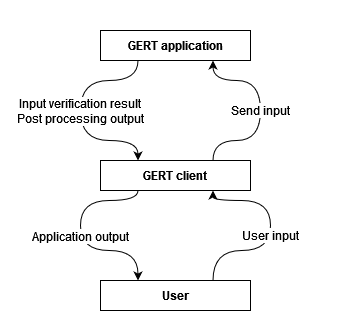
\includegraphics[width=0.75\linewidth]{REV0/SRS/gertcontextdiagram.png}
    	    \caption{Context Diagram}
    	    \label{fig: Context Diagram}
    	\end{center}
\end{figure}

\subsubsection{Work Partitioning}
\begin{table}[H]
    \centering
    \begin{tabular}{|p{4cm}|p{4cm}|p{6cm}|}
         \hline
         Event Name & Input and Output & Summary\\
         \hline
         User requests processed gps data & Input: CSV file Output: CSV file & System outputs normalized GPS data\\
         \hline
         User requests GPS episode extraction and mode detection & Input CSV file of gps data, Output: CSV file of of GPS episodes & System outputs episode extraction and mode detection CSV file\\
         \hline
         User requests trip segments based on processed data & Input: CSV file, Output: .shp file & System outputs GPS trip trajectories in a readable format for the user\\
         \hline
         User requests route choice sets & Input: .shp file, Output: .shp file & System outputs route choice sets and allows filtering based on set qualifiers\\
         \hline
         User requests activity locations  & Input: csv file, Output: .shp file & System outputs activity locations(stops) .shp file\\
         \hline
         User requests route choice analysis variables  & Input: .shp file, Output: .shp file & System outputs the route choice analysis variables along with justification for user perusal \\
         \hline
          User requests activity location identification  & Input: csv file, .shp file, .shp file, Output: .shp file& System outputs Activity location with Land Use and potential activity locations information in .shp file. \\
         \hline
    \end{tabular}
    \caption{Work Partitioning Diagram}
    \label{tab:team_roles}
\end{table}

\subsubsection{Product Boundary}

N/A

\subsubsection{Product Use Case List}
\begin{figure}[H]
	    \begin{center}
    	    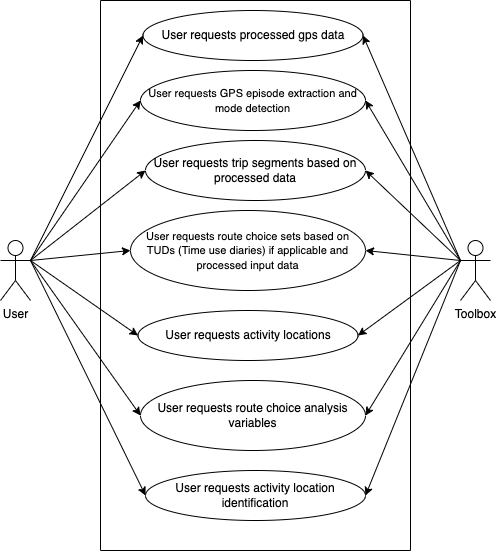
\includegraphics[width=1\linewidth]{REV0/SRS/useCaseDiagram.png}
    	    \caption{Use Case Diagram for Toolbox}
    	    \label{fig:Toolbox Use Case Diagram}
    	\end{center}
\end{figure}

\newpage

\subsubsection{Individual Product Use Cases}


\begin{itemize}
    \item[UC\refstepcounter{ucnum}\theucnum
\label{UC_Inputs_1}:] \plt{ Name: Process GPS data\\
        Trigger: User requests processed GPS data\\
        Preconditions: User has a csv file of unprocessed GPS data \\
        Stakeholders: User, Professor, Geospatial Analyst\\
        Actors:User, Toolbox\\
        Outcome: System outputs a csv file of normalized GPS data\\}
    \item[UC\refstepcounter{ucnum}\theucnum
\label{UC_Inputs_2}:] \plt{ Name: Episode extraction and mode detection\\
        Trigger: User requests GPS episode extraction and mode detection\\
        Preconditions: User has already requested processed GPS data \\
        Stakeholders: User, Professor, Geospatial Analyst\\
        Actors:User, Toolbox\\
        Outcome: System presents user with a csv file including all the episodes and mode detection data in a csv file\\}
    \item[UC\refstepcounter{ucnum}\theucnum
\label{UC_Inputs_3}:] \plt{ Name: Trip segment generation\\
        Trigger: User requests trip segments\\
        Preconditions: System has preprocessed input GPS data, user may optionally input TUD (time use diary) episodes\\
        Stakeholders: User, Professor, Geospatial Analyst\\
        Actors: User, Toolbox\\
        Outcome: .shp file with GPS trip trajectories in a readable format for the user\\}
    \item[UC\refstepcounter{ucnum}\theucnum
\label{UC_Inputs_4}:] \plt{ Name: Route choice set generation\\
        Trigger: User requests route choice sets\\
        Preconditions: System has preprocessed input GPS data and generated trip trajectories file\\
        Stakeholders: User, Professor, Geospatial Analyst\\
        Actors:User, Toolbox\\
        Outcome: .shp file with route choice sets\\}
    \item[UC\refstepcounter{ucnum}\theucnum
\label{UC_Inputs_5}:] \plt{ Name: Activity locations\\
        Trigger: User requests activity locations\\
        Preconditions: System has preprocessed input GPS data and extracted episodes and mode detection csv file \\
        Stakeholders: User, Professor, Geospatial Analyst\\
        Actors:User, Toolbox\\
        Outcome: System generates .shp file of activity locations (stops)\\}
    \item[UC\refstepcounter{ucnum}\theucnum
\label{UC_Inputs_6}:] \plt{ Name: Route choice analysis variable generation\\
        Trigger: User requests route choice analysis variables\\
        Preconditions: System has preprocessed input GPS data and generated trip trajectories file\\
        Stakeholders: User, Professor, Geospatial Analyst\\
        Actors:User, Toolbox\\
        Outcome: .csv file containing route choice analysis variables and variable justification\\}
    \item[UC\refstepcounter{ucnum}\theucnum
\label{UC_Inputs_7}:] \plt{ Name: Activity location identification\\
        Trigger:User has requested activity location identification\\
        Preconditions: System has preprocessed input GPS data, extracted episodes and mode detection csv file, and then extracted activity location .shp file, as well as user has inputted land use .shp file potential activity location .shp file \\
        Stakeholders: User, Professor, Geospatial Analyst\\
        Actors:User, Toolbox\\
        Outcome: System outputs a .shp file of activity location with land use and potential activity location information .shp file\\}
\end{itemize}

\subsection{Functional and Data Requirements}
\noindent \begin{itemize}

\item[R\refstepcounter{reqnum}\thereqnum
\label{R_Inputs_1}:] \plt{The system shall allow users to upload GPS data in standard format.}
\begin{itemize}
    \item \textbf{Requirement Type}: Functional
    \item \textbf{Rationale}: The user needs to upload GPS data for processing.
    \item \textbf{Fit Criterion}: The system successfully uploads the file and notifies the user.
    \item \textbf{Priority}: 5
    \item \textbf{Event}: UC1
    \item \textbf{Customer Satisfaction}: 5
    \item \textbf{Customer Dissatisfaction}: 5
    \item \textbf{Conflict}:None
    \item \textbf{Planned Date}: November 14, 2022
\end{itemize}

\item[R\refstepcounter{reqnum}\thereqnum
\label{R_Inputs_1}:] \plt{The system shall process GPS data points.}
\begin{itemize}
    \item \textbf{Requirement Type}: Data
    \item \textbf{Rationale}: System must analysis activity data.
    \item \textbf{Fit Criterion}: The system outputs GPS data points as latitude, longtude, and time variables. 
    \item \textbf{Priority}: 5
    \item \textbf{Event}: UC1
    \item \textbf{Customer Satisfaction}: 5
    \item \textbf{Customer Dissatisfaction}: 5
    \item \textbf{Conflict}: R1.
    \item \textbf{Planned Date}: November 14, 2022
\end{itemize}

\item[R\refstepcounter{reqnum}\thereqnum
\label{R_Inputs_1}:] \plt{The system shall accept TUD data points.}
\begin{itemize}
    \item \textbf{Requirement Type}: Data
    \item \textbf{Rationale}: System must analysis activity data.
    \item \textbf{Fit Criterion}: User successfully upload TUD data in standard format such as csv. 
    \item \textbf{Priority}: 5
    \item \textbf{Event}: UC3
    \item \textbf{Customer Satisfaction}: 5
    \item \textbf{Customer Dissatisfaction}: 5
    \item \textbf{Conflict}: None
    \item \textbf{Planned Date}: November 14, 2022
\end{itemize}

\item[R\refstepcounter{reqnum}\thereqnum
\label{R_Output_3}:] \plt{The system shall produce output in a standard transferable format.}
\begin{itemize}
    \item \textbf{Requirement Type}: Functional
    \item \textbf{Rationale}: User must read data and re-use output data across multiple applications.
    \item \textbf{Fit Criterion}: System successfully outputs data in standard format such as csv. 
    \item \textbf{Priority}: 5
    \item \textbf{Event}: UC1-7
    \item \textbf{Customer Satisfaction}: 5
    \item \textbf{Customer Dissatisfaction}: 4
    \item \textbf{Conflict}: None
    \item \textbf{Planned Date}: November 14, 2022
\end{itemize}

\item[R\refstepcounter{reqnum}\thereqnum
\label{R_Inputs_2}:] \plt{The system shall use longitude, latitude, and time variables from GPS data points.}
\begin{itemize}
    \item \textbf{Requirement Type}: Data
    \item \textbf{Rationale}: System must use general variables to make computations and produce analysis.
    \item \textbf{Fit Criterion}: System successfully extracts longitude, latitude, and time information from inputs.
    \item \textbf{Priority}: 5
    \item \textbf{Event}: UC1-7
    \item \textbf{Customer Satisfaction}: 5
    \item \textbf{Customer Dissatisfaction}: 5
    \item \textbf{Conflict}: R2
    \item \textbf{Planned Date}: November 14, 2022
\end{itemize}

\item[R\refstepcounter{reqnum}\thereqnum
\label{R_Outputs_1}:] \plt{The system shall extract episode attributes including speed, duration, direction, distance, change in direction, acceleration, and status points from GPS data points.}
\begin{itemize}
    \item \textbf{Requirement Type}: Functional
    \item \textbf{Rationale}: System must categorize data points to useful information for the user to read.
    \item \textbf{Fit Criterion}: System successfully produce reports of episode attributes. 
    \item \textbf{Priority}: 5
    \item \textbf{Event}: UC2
    \item \textbf{Customer Satisfaction}: 5
    \item \textbf{Customer Dissatisfaction}: 5
    \item \textbf{Conflict}: R5
    \item \textbf{Planned Date}: November 14, 2022
\end{itemize}

\item[R\refstepcounter{reqnum}\thereqnum
\label{R_Inputs_1}:] \plt{The system shall extract episode attributes including duration, distance, and change in trajectory from TUD data points.}
\begin{itemize}
    \item \textbf{Requirement Type}: Functional
    \item \textbf{Rationale}: The system needs to validate  analysis of GPS points.
    \item \textbf{Fit Criterion}: System successfully produce reports of episode attribute.
    \item \textbf{Priority}: 5
    \item \textbf{Event}: UC3
    \item \textbf{Customer Satisfaction}: 5
    \item \textbf{Customer Dissatisfaction}: 4
    \item \textbf{Conflict}: R3
    \item \textbf{Planned Date}: November 14, 2022
\end{itemize}

\item[R\refstepcounter{reqnum}\thereqnum
\label{R_Inputs_1}:] \plt{The system shall classify extracted episode into different types including stop, car, walk, bus, and other travel episodes.}
\begin{itemize}
    \item \textbf{Requirement Type}: Functional
    \item \textbf{Rationale}: User need to understand travel behaviour of objects' episode.  
    \item \textbf{Fit Criterion}: System successfully classify predefined examples into correct episode types. 
    \item \textbf{Priority}: 5
    \textbf{Event}: UC2
    \item \textbf{Customer Satisfaction}: 5
    \item \textbf{Customer Dissatisfaction}: 5
    \item \textbf{Conflict}: R6,7
    \item \textbf{Planned Date}: November 14, 2022
\end{itemize}

\item[R\refstepcounter{reqnum}\thereqnum
\label{R_Outputs_2}:] \plt{The system shall decompose episode into output segments of type stop and trip.}
\begin{itemize}
    \item \textbf{Requirement Type}: Functional
    \item \textbf{Rationale}: User need to understand the object's behaviour during a segment.
    \item \textbf{Fit Criterion}: System successfully categorize a moving object in a trip segment and a static object in stop segment
    \item \textbf{Priority}: 5
    \item \textbf{Event}: UC3
    \item \textbf{Customer Satisfaction}: 5
    \item \textbf{Customer Dissatisfaction}: 5
    \item \textbf{Conflict}: R8
    \item \textbf{Planned Date}: November 14, 2022
\end{itemize}

\item[R\refstepcounter{reqnum}\thereqnum
\label{R_Inputs_1}:] \plt{The system shall identify trip trajectory using extracted segments.}
\begin{itemize}
    \item \textbf{Requirement Type}: Functional
    \item \textbf{Rationale}: The system needs trip trajectory for route analysis. 
    \item \textbf{Fit Criterion}: The system successfully identifies the change in the trajectory when the object changes direction. 
    \item \textbf{Priority}: 5
    \item \textbf{Event}: UC3,4
    \item \textbf{Customer Satisfaction}: 5
    \item \textbf{Customer Dissatisfaction}: 5
    \item \textbf{Conflict}: R9
    \item \textbf{Planned Date}: November 14, 2022
\end{itemize}

\item[R\refstepcounter{reqnum}\thereqnum
\label{R_Inputs_1}:] \plt{The system shall identify activity locations based on the episode attributes of the route to the stop point.}
\begin{itemize}
    \item \textbf{Requirement Type}: Functional
    \item \textbf{Rationale}: The system needs location types for land use and road network analysis.
    \item \textbf{Fit Criterion}: The system successfully identify a high activity locations and low activity locations. 
    \item \textbf{Priority}: 5
    \item \textbf{Event}: UC5,7
    \item \textbf{Customer Satisfaction}: 5
    \item \textbf{Customer Dissatisfaction}: 5
    \item \textbf{Conflict}: R6,7
    \item \textbf{Planned Date}: November 14, 2022
\end{itemize}

\item[R\refstepcounter{reqnum}\thereqnum
\label{R_Inputs_1}:] \plt{The system shall generate RCA variables based on trip trajectory.}
\begin{itemize}
    \item \textbf{Requirement Type}: Functional
    \item \textbf{Rationale}: The system needs to define route choice behaviour data set.
    \item \textbf{Fit Criterion}: The system successfully defines variables to describe a route from position A to position B.
    \item \textbf{Priority}: 5
    \item \textbf{Event}: UC4,6
    \item \textbf{Customer Satisfaction}: 5
    \item \textbf{Customer Dissatisfaction}: 4
    \item \textbf{Conflict}: R10
    \item \textbf{Planned Date}: November 14, 2022
\end{itemize}


\item[R\refstepcounter{reqnum}\thereqnum
\label{R_Inputs_1}:] \plt{The system shall store RCA data set.}
\begin{itemize}
    \item \textbf{Requirement Type}: Data
    \item \textbf{Rationale}: The system needs to track the RCA for descriptive route analysis. 
    \item \textbf{Fit Criterion}: System successfully stored multiple instances of RCA variables. 
    \item \textbf{Priority}: 4
    \item \textbf{Event}: UC4,6
    \item \textbf{Customer Satisfaction}: 5
    \item \textbf{Customer Dissatisfaction}: 4
    \item \textbf{Conflict}: R12
    \item \textbf{Planned Date}: November 14, 2022
\end{itemize}

\item[R\refstepcounter{reqnum}\thereqnum
\label{R_Inputs_1}:] \plt{The system shall automate routes from position A to position B based on RCA set.}
\begin{itemize}
    \item \textbf{Requirement Type}: Functional
    \item \textbf{Rationale}: The user wants to request routes from position A to position B.
    \item \textbf{Fit Criterion}: The system produce a mapped route from position A to position B.
    \item \textbf{Priority}: 4
    \item \textbf{Event}: UC6
    \item \textbf{Customer Satisfaction}: 5
    \item \textbf{Customer Dissatisfaction}: 4
    \item \textbf{Conflict}: R13
    \item \textbf{Planned Date}: November 14, 2022
\end{itemize}

\item[R\refstepcounter{reqnum}\thereqnum
\label{R_Inputs_1}:] \plt{The system shall allow users to select options for automated route requests.}
\begin{itemize}
    \item \textbf{Requirement Type}: Functional
    \item \textbf{Rationale}: The user needs the option to customize routes. 
    \item \textbf{Fit Criterion}: The system successfully maps a route with selected options such as shortest distance. 
    \item \textbf{Priority}: 4
    \item \textbf{Event}: UC6
    \item \textbf{Customer Satisfaction}: 4
    \item \textbf{Customer Dissatisfaction}: 4
    \item \textbf{Conflict}: R13
    \item \textbf{Planned Date}: November 14, 2022
\end{itemize}

\item[R\refstepcounter{reqnum}\thereqnum
\label{R_Inputs_1}:] \plt{The system shall store activity location identifications.}
\begin{itemize}
    \item \textbf{Requirement Type}: Data
    \item \textbf{Rationale}: The user needs to search for specific type of activity location.
    \item \textbf{Fit Criterion}: The system successfully stores data and notifies user. 
    \item \textbf{Priority}:4
    \item \textbf{Event}: UC5,7
    \item \textbf{Customer Satisfaction}: 4
    \item \textbf{Customer Dissatisfaction}: 2
    \item \textbf{Conflict}: R11
    \item \textbf{Planned Date}: November 14, 2022
\end{itemize}

\item[R\refstepcounter{reqnum}\thereqnum
\label{R_Inputs_1}:] \plt{The system shall classify RCA patterns by route purpose.}
\begin{itemize}
    \item \textbf{Requirement Type}: Functional
    \item \textbf{Rationale}: The system needs to define trip purpose.
    \item \textbf{Fit Criterion}: The system successfully defines purpose of a route from position A to position B.
    \item \textbf{Priority}: 5
    \item \textbf{Event}: UC4,6
    \item \textbf{Customer Satisfaction}: 5
    \item \textbf{Customer Dissatisfaction}: 4
    \item \textbf{Conflict}: R16,13
    \item \textbf{Planned Date}: November 14, 2022
\end{itemize}

\item[R\refstepcounter{reqnum}\thereqnum
\label{R_Inputs_1}:] \plt{The system shall allows requests for activity location description by filtering.}
\begin{itemize}
    \item \textbf{Requirement Type}: Functional
    \item \textbf{Rationale}: The user needs the options to search for specific type of activity location.
    \item \textbf{Fit Criterion}: The system successfully outputs relevant types of activity locations to what the user requested. 
    \item \textbf{Priority}:4
    \item \textbf{Event}: UC5,7
    \item \textbf{Customer Satisfaction}: 4
    \item \textbf{Customer Dissatisfaction}: 2
    \item \textbf{Conflict}: R16
    \item \textbf{Planned Date}: November 14, 2022
\end{itemize}

\item[R\refstepcounter{reqnum}\thereqnum
\label{R_Inputs_1}:] \plt{The system shall allow users to request trip segments' description for a given GPS data set.}
\begin{itemize}
    \item \textbf{Requirement Type}: Functional
    \item \textbf{Rationale}: The user needs to review intermediate analysis steps. 
    \item \textbf{Fit Criterion}: The system successfully produce trip segment reports. 
    \item \textbf{Priority}: 5
    \item \textbf{Event}: UC3
    \item \textbf{Customer Satisfaction}: 5
    \item \textbf{Customer Dissatisfaction}: 5
    \item \textbf{Conflict}: R9
    \item \textbf{Planned Date}: November 14, 2022
\end{itemize}

\item[R\refstepcounter{reqnum}\thereqnum
\label{R_Inputs_1}:] \plt{The system shall allow users to request episode descriptions of GPS inputs.}
\begin{itemize}
    \item \textbf{Requirement Type}: Functional
    \item \textbf{Rationale}: The user needs to access intermediate details about episode attributes.
    \item \textbf{Fit Criterion}: The system successfully produces a standard output file with the requested details.
    \item \textbf{Priority}: 5
    \item \textbf{Event}: UC2
    \item \textbf{Customer Satisfaction}: 5
    \item \textbf{Customer Dissatisfaction}: 5
    \item \textbf{Conflict}: R6-8
    \item \textbf{Planned Date}: November 14, 2022
\end{itemize}

\end{itemize}

\section{Non-functional Requirements}

\subsection{Look and Feel Requirements}

\subsection{Usability and Humanity Requirements}

\subsection{Performance Requirements}

\subsection{Operational and Environmental Requirements}

\subsection{Maintainability and Support Requirements}

\subsection{Security Requirements}

\subsection{Cultural Requirements}

\subsection{Legal Requirements}

\subsection{Health and Safety Requirements}

This section is not in the original Volere template, but health and safety are
issues that should be considered for every engineering project.

\section{Project Issues}

\subsection{Open Issues}

\subsection{Off-the-Shelf Solutions}

\subsection{New Problems}

\subsection{Tasks}

\subsection{Migration to the New Product}

\subsection{Risks}

\subsection{Costs}

\subsection{User Documentation and Training}

\subsection{Waiting Room}

\subsection{Ideas for Solutions}

\bibliographystyle{plainnat}

\bibliography{SRS}

\newpage

\section{Appendix}

This section has been added to the Volere template.  This is where you can place
additional information.

\subsection{Symbolic Parameters}

The definition of the requirements will likely call for SYMBOLIC\_CONSTANTS.
Their values are defined in this section for easy maintenance.


\end{document}
